\chapter{実験}
\label{sq:Experiments}

我々のタスクには公開されたデータセットが存在しないため,
まずデータセットの作成の概略と統計情報について説明する.
それからベースライン手法を含む実験設定について紹介し最後に実験結果を示す.

\section{データセット}

Webや雑誌から自動,または,手動によって,
3クラスのエンティティに対する様々なエンティティ順序を抽出した.
これら3クラスは都道府県,国,カメラである.
クラス選定は以下の4つの理由に基づいた:
(1) 順序基準と特徴に関するWebページの量,
(2) エンティティ順序の種類数,
(3) 数値属性の量,
(4) 統計情報の多様性.

都道府県と国に関してはエンティティ列をWebページ中のランキング(各エンティティが1位,2位等に順位付けされているコンテンツ)から自動的に抽出した.
カメラに関しては,国内で発売されている10のカメラ雑誌からエンティティ順序を手動で抽出した.
このような雑誌には,各カメラに様々な観点から点数や順位が与えられているため,
それらに基づいてエンティティ列を構築した.
上記の結果として得られたエンティティ列はそれぞれエンティティペアに変換され,
部分的に観測された順序集合$O_{\preceq_{k}}$を得た.
要素数が5未満であった順序集合を除き,最終的に158のエンティティ順序を得た.

都道府県と国の数値属性はWeb上で公開されているものを自動的に抽出し,
カメラについては価格.com\footnote{\url{http://kakaku.com/}}のページよりスペック情報などを抽出し数値属性とした.
数値属性を抽出後に,各属性ごとに$[0, 1]$に収まるよう各属性の最大値と最小値によって正規化を行った.

\begin{table}[t]
\centering
\caption{各クラスの統計情報とエンティティ,エンティティ順序,および,属性の例.}
\begin{tabular}{l p{5em} p{5em} p{5em}}
\toprule
&都道府県&国&カメラ\\
\midrule
\# Entities&47&138&149\\
\# Orders&64&40&54\\
\# Entities / Order&13.3&17.7&14.4\\
\# Attributes&137&83&16\\
(\# Entities / Order)&\multirow{2}{*}{0.097}&\multirow{2}{*}{0.213}&\multirow{2}{*}{0.900}\\
\hspace{1em}/ \# Attributes&\\
\midrule
\multirow{2}{*}{Entity examples}&\multicolumn{1}{l}{東京}&\multicolumn{1}{l}{デンマーク}&\multicolumn{1}{l}{EOS 5DS}\\
&\multicolumn{1}{l}{京都}&\multicolumn{1}{l}{アイスランド}&\multicolumn{1}{l}{Nikon D3300}\\
\midrule
\multirow{2}{*}{Attribute examples}&\multicolumn{1}{l}{人口}&\multicolumn{1}{l}{旅行者数}&\multicolumn{1}{l}{解像度}\\
&\multicolumn{1}{l}{犯罪率}&\multicolumn{1}{l}{自殺者数}&\multicolumn{1}{l}{重さ}\\
\midrule
\multirow{2}{*}{Order examples}&\multicolumn{1}{l}{魅力度}&\multicolumn{1}{l}{住みやすさ}&\multicolumn{1}{l}{持ち運びやすさ}\\
&\multicolumn{1}{l}{豊かさ}&\multicolumn{1}{l}{幸福度}&\multicolumn{1}{l}{耐久性}\\
\bottomrule
\end{tabular}

\label{tb:statistics}
\end{table}

表\ref{tb:statistics}に統計情報とエンティティ,エンティティ順序,および,属性の例を示す.
多くのエンティティ順序に対して,我々はすべてのエンティティを含むようなランキングを見つけることができなかった.
これは,それらのページが上位1,3,5件のみを紹介することが多かったためである.
また,表中に示されている統計値の中で最も重要な値は属性数に対する1エンティティ順序あたりのエンティティ数の比率である((\# Entities / Order) / \# Attributes).
この比率は全てのクラスで1.0以下であり,
カメラクラスが最も高く,都道府県クラスが最も低くなっている.

\section{実験設定}

我々は実験におけるベースライン手法として,
文脈を用いない既存のランキング学習手法を用いた:
(1) {\bf RankNet}~\cite{burges2005learning}: ニューラルネットワークを用いクロスエントロピー損失を最適化するペアワイズランキング手法,
(2) {\bf RankBoost}~\cite{freund2003efficient}: AdaBoost~\cite{freund1997decision}のペアワイズランキングへの応用,
(3) {\bf LinearFeature}~\cite{metzler2007linear}: 座標上昇法によって最適化された線形特徴モデル,
(4) {\bf LambdaMART}~\cite{wu2010adapting}: ランキング学習手法であるLambdaRank~\cite{burges2006learning}と決定木ブースティングモデルであるMART~\cite{friedman2001greedy}を組み合わせた手法,
(5) {\bf ListNet}~\cite{cao2007learning}: ニューラルネットワークを用いたリストワイズランキング手法.
我々はRankLib\footnote{\url{https://sourceforge.net/p/lemur/wiki/RankLib/}}での実装を実験に用いた.
なお,タスクが互いに関連しているという仮定をしなかったため,マルチタスク学習との比較は行わなかった.

構築したデータセットを用いた実験の手順を以下で述べる.
各順序集合$O_{\preceq_{k}}$に対し,
$O_{\preceq_{k}}$に含まれるエンティティ集合$E$を1対1に分割し,
これらを$E_{\rm train}$および$E_{\rm test}$とした.
訓練データは$O_{\rm train} = \{(e_i, e_j) | (e_i, e_j) \in O_{\preceq_{k}} \wedge e_i \in E_{\rm train} \wedge e_j \in E_{\rm train} \}$であり,
テストデータは$O_{\rm test} = O_{\preceq_{k}} - O_{\rm train}$とした.
実験でのタスクは,$O_{\rm train}$に基づいて順序モデルを学習し,
各$(e_i, e_j) \in O_{\rm test}$に対して$e_i$と$e_j$のどちらが上位に順序づけされるかを予測する問題とした.
この問題において,精度は正しく予測できたエンティティペア数と定義された.
我々はあるクラスにおけるエンティティ順序に対して,5分割交差法を用いて各手法の最適なパラメータを決定した.

文脈誘導型学習({\bf CGL})では以下の設定を用いた.
文脈モデルとして{\bf TF-IDF}と{\bf Distributed} ($L=400$の分散表現)を用いた.
パラメータ$c$と$C$は上述の交差法を用いて決定された.

\section{実験結果}

\begin{table}[t]
\centering
\caption{各ランキング手法の精度 ($\pm$標準誤差).
太字は各エンティティクラスでの最大の精度を表す.}
\begin{tabular}{l c c c p{0.1em} c }
\toprule
&\multicolumn{5}{c}{精度}\\
\cmidrule(lr){2-6}
&都道府県&国&カメラ&&総合\\
\midrule
\multirow{2}{*}{RankNet~\cite{burges2005learning}}&0.482 & 0.478 & 0.530 && 0.497 \\ 
& (0.023) & (0.025) & (0.030) && (0.015) \\
\midrule
\multirow{2}{*}{RankBoost~\cite{freund2003efficient}}&0.513 & 0.636 & 0.552 && 0.557 \\
 & (0.028) & (0.024) & (0.036) && (0.018) \\
\midrule
\multirow{2}{*}{LinearFeature~\cite{metzler2007linear}}&0.566 & 0.670 & 0.614 && 0.609 \\
 & (0.019) & (0.024) & (0.034) && (0.015) \\
\midrule
\multirow{2}{*}{LambdaMART~\cite{wu2010adapting}}&0.614 & 0.659 & 0.697 && 0.654 \\
 & (0.021) & (0.019) & (0.024) && (0.013) \\
\midrule
\multirow{2}{*}{ListNet~\cite{cao2007learning}}&0.559 & 0.518 & 0.504 && 0.530 \\
 & (0.020) & (0.022) & (0.031) && (0.014) \\
\midrule
\midrule
\multirow{2}{*}{{\bf CGL} (TF-IDF, Linear)}&{\bf 0.661} & 0.716 & {\bf 0.823} && {\bf 0.730} \\
 & (0.017) & (0.022) & (0.019) && (0.012) \\
\midrule
\multirow{2}{*}{{\bf CGL} (TF-IDF, RBF)}&{\bf 0.661} & 0.725 & 0.799 && 0.724 \\
 & (0.019) & (0.021) & (0.019) && (0.012) \\
\midrule
\multirow{2}{*}{{\bf CGL} (Distributed, Linear)}& 0.646 & 0.701 & 0.798 && 0.712 \\
 & (0.020) & (0.023) & (0.021) && (0.013) \\
\midrule
\multirow{2}{*}{{\bf CGL} (Distributed, RBF)}&{\bf 0.661} & {\bf 0.731} & 0.804 && 0.728 \\
 & (0.018) & (0.022) & (0.021) && (0.013) \\
\bottomrule
\end{tabular}
\label{tb:real_data_results}
\end{table}

表\ref{tb:real_data_results}に精度と標準誤差を示す.
文脈誘導型学習(CGL)はどの設定においてもベースライン手法を上回る精度を達成している.文脈誘導型学習に基づいた手法の中で最も精度の高かった手法はCGL (TF-IDF, Linear)であり,次点はCGL (Distributed, RBF)であった.
最も精度の高いベースライン手法であるLambdaMartからの
総合的な精度改善は11.6\%であった.
ランダム化Tukey HSDテスト~\cite{carterette2012multiple}\footnote{\url{http://www.f.waseda.jp/ tetsuya/tools.html}}($\alpha = 0.01$)によれば,
CGL (TF-IDF, Linear)と全ベースライン手法との差は統計的有意であり,
文脈誘導型学習に基づいた手法の中では統計的有意差は認められなかった.

クラスごとに見ると,都道府県,国,カメラクラスにおいて,
CGL (TF-IDF, Linear)はLambdaMARTの精度をそれぞれ8\%,11\%,18\%改善した.
我々は,事前に行った人工データでの実験と文脈モデルに用いられた1属性当たりの文数がそれぞれ36.0,45.7,137であったことから,
文脈の質と量が文脈誘導型学習の効果を決定する主な要因ではないかと考えている.

我々は学習された関数内で用いられている属性の評価も行った.
最も絶対値の高い重みを持つ5つの属性をエンティティ順序ごとにプールし,
クラウドソーシングサービスLancers\footnote{\url{http://www.lancers.jp/}}のユーザに対して提示した.
この実験では学習された属性がどの程度順序を説明できるのかを理解することを目的としている.
ユーザは与えられた順序基準と属性の間に相関があるかどうかを,
$-2$から$+2$までの5段階で評価した.
我々は各順序基準と属性のペアに対して5名のユーザを割り当てた.
最も精度の高かったCGL (TF-IDF, Linear)とベースライン中で唯一線形関数を用いるLinearFeatureが評価に選ばれた.

\begin{figure}[t]
  \begin{center}
    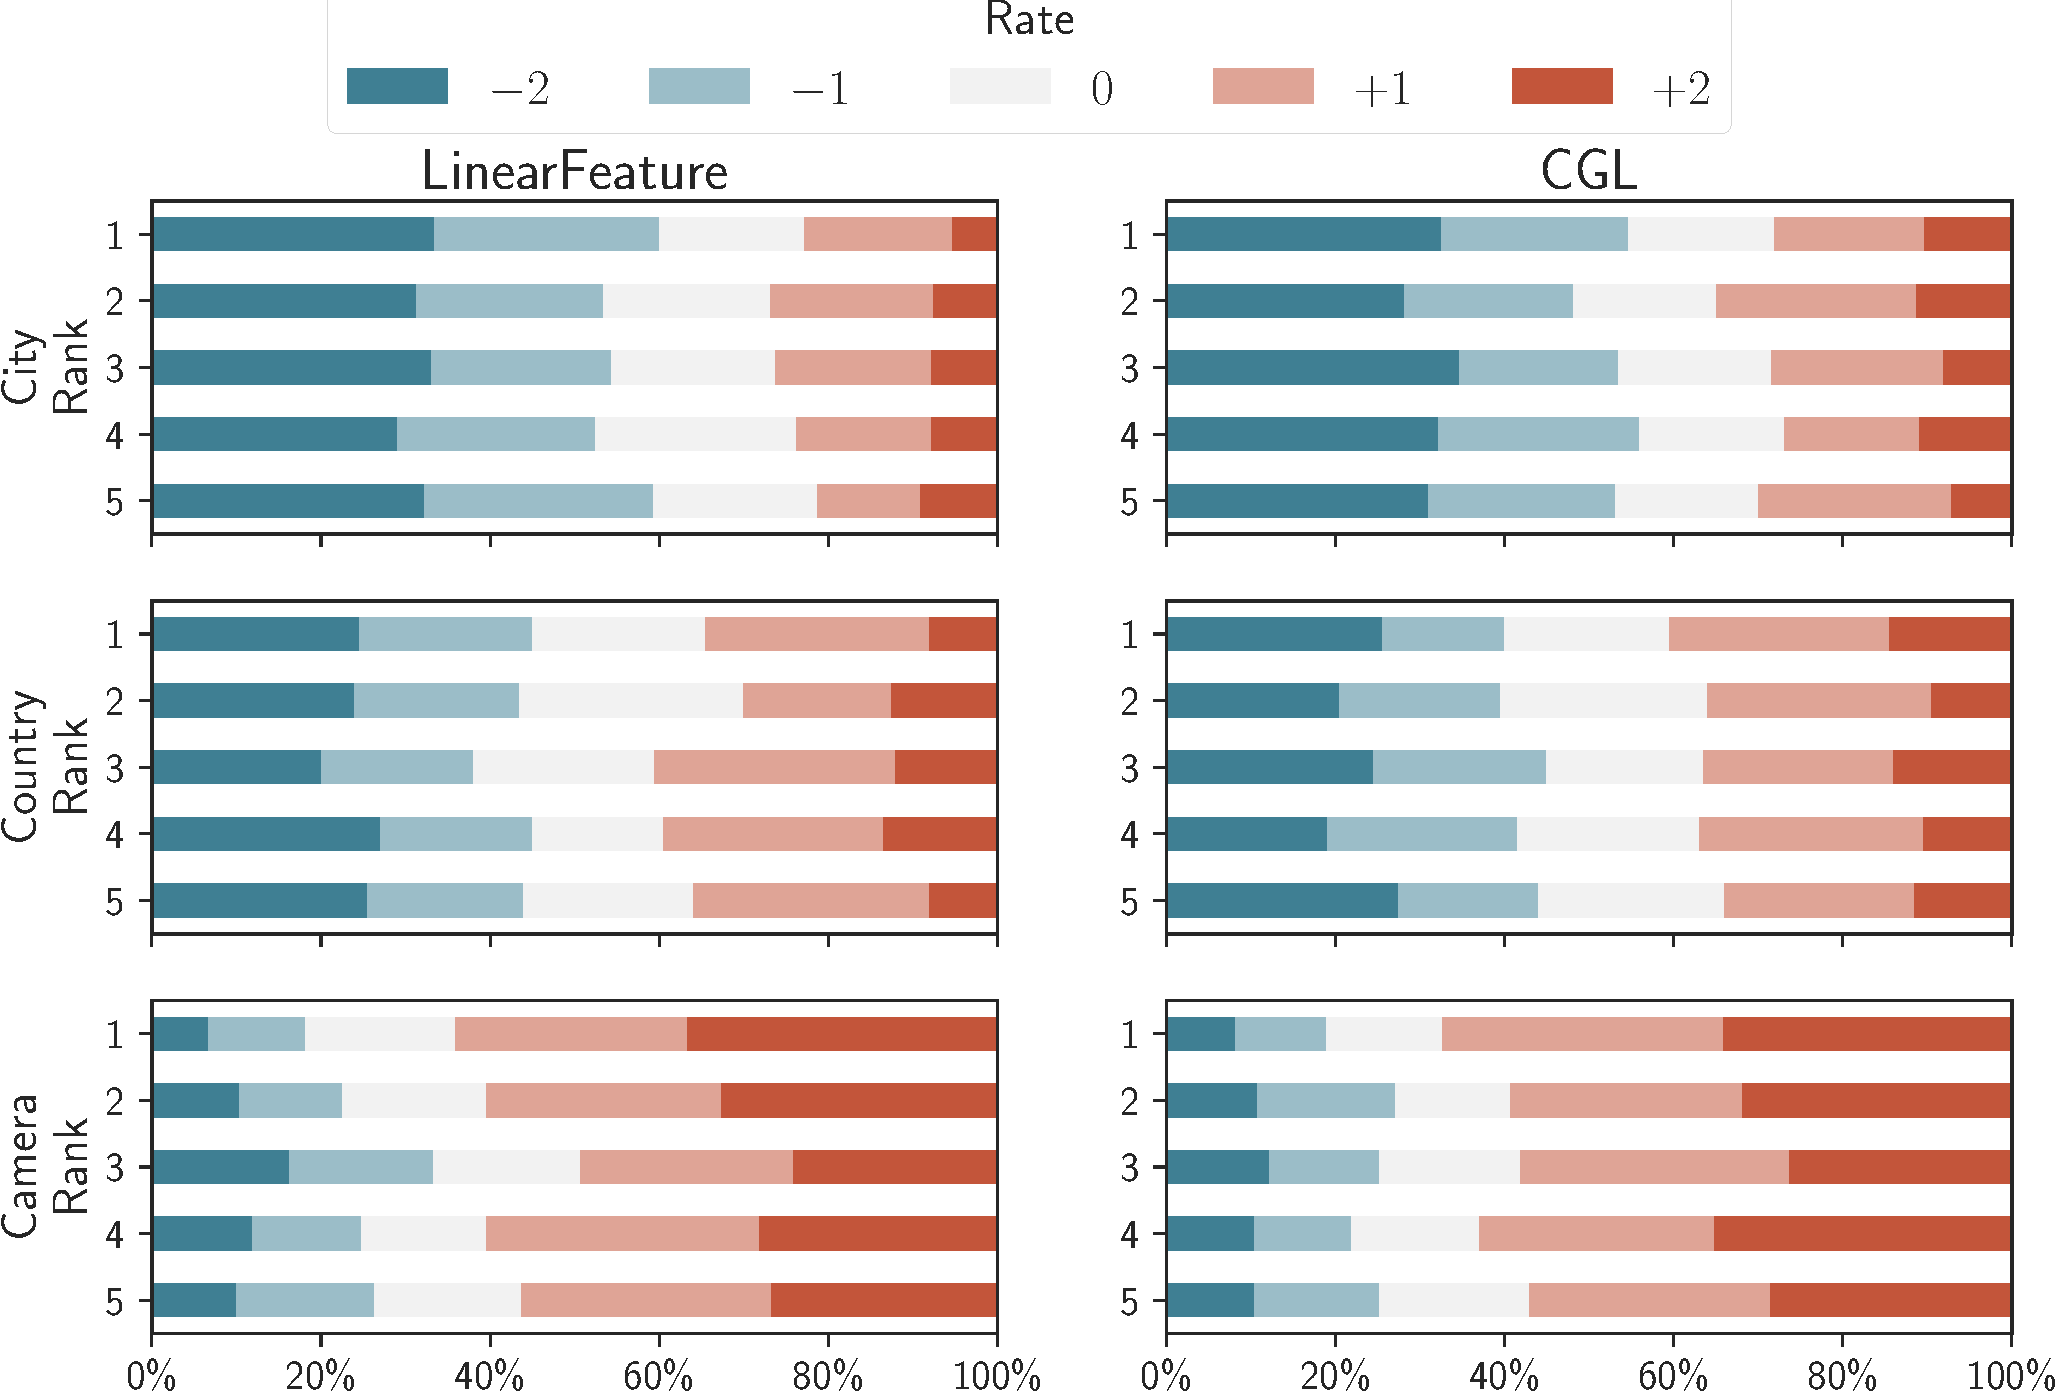
\includegraphics[width=\columnwidth]{images/rates}
    \caption{最も絶対値の高い重みを持つ5つの属性の評価値の分布.}
    \label{fig:weights_evaluation_results}
  \end{center}
\end{figure}

図\ref{fig:weights_evaluation_results}に最も絶対値の高い重みを持つ5つの属性の評価値の分布を示す.
都道府県,国,カメラに対して,文脈誘導型学習の平均評価値はそれぞれ,
$-0.455$,$-0.166$,$+0.581$であり,
LinearFeatureの平均評価値はそれぞれ,$-0.560$,$-0.204$,$+0.516$であった.
これらの評価値は手法の精度と高い相関がある.
文脈誘導型学習はすべてのクラスにおいてLinearFeatureよりも妥当な属性を発見できていたが,全てのクラスにおいてその差はわずかである.
都道府県と国における平均評価値は0以下となっており,各属性の低い説明可能性を示唆している.
これは単に各属性が順序基準と相関があったものの,
順序基準に変化をもたらす要因として評価されなかったためではないかと考えている.
文脈誘導型学習はベースラインよりも精度が高いモデルを学習できたものの,
与えられた順序基準に対して高い説明可能性を持った属性を発見するのは未だ挑戦的な課題であると言える.

\begin{table}[t]
\centering
\caption{文脈誘導型学習によって学習された線形関数の例.最も絶対値の高い重みを持つ3つの属性のみを示している.
}
\scalebox{0.725}{
\begin{tabular}{l p{1em} l c c l c l c l }
\toprule
クラス&&\multicolumn{8}{c}{学習された線型モデル}\\
\midrule
都道府県&&魅力度&$=$&$+0.035$&女性の平均寿命&$-0.032$&交通事故死者数&$-0.031$&人口/世帯数\\
都道府県&&貯蓄額&$=$&$-0.174$&最高気温&$+0.160$&健康寿命&$+0.148$&旅館数\\
国&&評判&$=$&$+0.058$&幸福度 &$-0.057$&難民申請数& $-0.045$&自殺者数\\
国&&平和&=&$+0.170$&穀物収穫量&$+0.166$&GDP成長率&$-0.126$&自殺者数\\
カメラ&&操作性&$=$&$-0.240$&重さ&$-0.213$&高さ&$+ 0.133$&シャッタースピード\\
\bottomrule
\end{tabular}
}
\label{tb:learnt_models}
\end{table}

最後に,文脈誘導型学習によって学習された線形関数の例を表\ref{tb:learnt_models}に示す.
多くの属性はエンティティ順序を説明可能で影響を与えているように見える.
一方,いくつかの属性はエンティティ順序を説明するために適切でないように見えるが(例えば,``魅力度''に対する``世帯当たりの人口''や``貯蓄額''に対する``最高気温''),
データセット中ではエンティティ順序と高い相関を示している.
これらは主観的評価では妥当でないと判断されたものの,
予測においては大きく貢献している属性の例である.

